\documentclass[margin=5mm]{standalone}
\usepackage[dvipsnames]{xcolor}
\usepackage{pgfplots}
\usepackage{tikz}

\pgfplotsset{compat=1.18}
\begin{document}

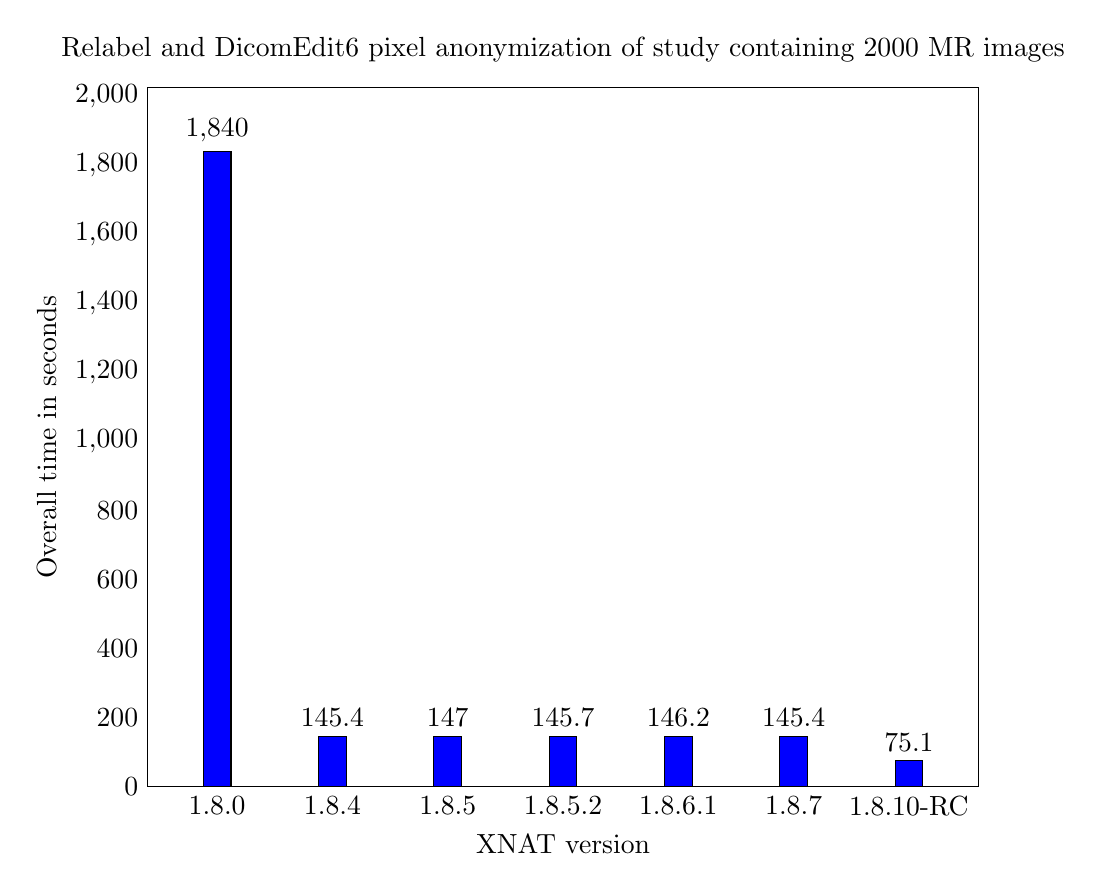
\begin{tikzpicture}
    \begin{axis}[
        width = \textwidth,
        xlabel = XNAT version,
        ylabel = Overall time in seconds,
        symbolic x coords = {1.8.0,1.8.4,1.8.5,1.8.5.2,1.8.6.1,1.8.7,1.8.10-RC},
        nodes near coords,
        xtick = {1.8.0,1.8.4,1.8.5,1.8.5.2,1.8.6.1,1.8.7,1.8.10-RC},
        ymin = 0,
        xtick pos = left,
        ytick pos = left,
        xticklabel style = {major tick length = 0pt},
        title = {Relabel and DicomEdit6 pixel anonymization of study containing 2000 MR images}]
        \addplot[ybar,fill=blue] coordinates {(1.8.0, 1840.0)};
        \addplot[ybar,fill=blue] coordinates {(1.8.4, 145.4)};
        \addplot[ybar,fill=blue] coordinates {(1.8.5, 147.0)};
        \addplot[ybar,fill=blue] coordinates {(1.8.5.2, 145.7)};
        \addplot[ybar,fill=blue] coordinates {(1.8.6.1, 146.2)};
        \addplot[ybar,fill=blue] coordinates {(1.8.7, 145.4)};
        \addplot[ybar,fill=blue] coordinates {(1.8.10-RC, 75.1)};
    \end{axis}
\end{tikzpicture}

\end{document}